\chapter{废物利用与物质循环再生}
\label{chp:recycling:begin}

舱内固体废物包括乘员及黄粉虫粪便、植物不可食部分、餐厨垃圾等,其处理和再利用与系统闭合度密切相关。因此,固体废物处理是生物再生生命保障系统中重要的单元。

\section{主选方案}

我们设计的火星宫采用微生物燃料电池。
微生物燃料电池(Microbial Fuel Cell,MFC)是一种利用微生物将有机物中的化学能直接转化成电能的装置。其基本工作原理是:在阳极室厌氧环境下,有机物在微生物作用下分解并释放出电子和质子,电子依靠合适的电子传递介体在生物组分和阳极之间进行有效传递,并通过外电路传递到阴极形成电流,而质子通过质子交换膜传递到阴极,氧化剂(一般为氧气)在阴极得到电子被还原与质子结合成水。
参与传递电子的介体与微生物和阳极之间的作用形式有三种:
\begin{enumerate}
  \item
    微生物将氧化还原反应产生的电子直接传递给溶解在溶液中的介体,介体再将电子传递给电极;
  \item
    介体能进入到微生物体内,参加反应被还原,从微生物体内出来后再将电子传递给电极;
  \item
微生物吸附在电极表面,它将反应产生的电子传递给在细胞表面的介体,再通过介体传递给电极。
\end{enumerate}

优势:
与现有的其它利用有机物产能的技术相比,微生物燃料电池具有操作上和功能上的优势: 首先,它将底物直接转化为电能,保证了具有高的能量转化效率; 其次,不同于现有的所有生物能处理,微生物燃料电池在常温环境条件下能够有效运作; 第三,微生物燃料电池不需要进行废气处理,因为它所产生的废气的主要组分是二氧化碳,二氧化碳还可以用作促进植物生长; 第四,微生物燃料电池不需要输入较大能量,因为若是单室微生物燃料电池仅需通风就可以被动的补充阴极气体。舱内所产生的大部分固体与液体废物绝大部分可以使用MFC处理。

\begin{figure}[H]
  \centering
  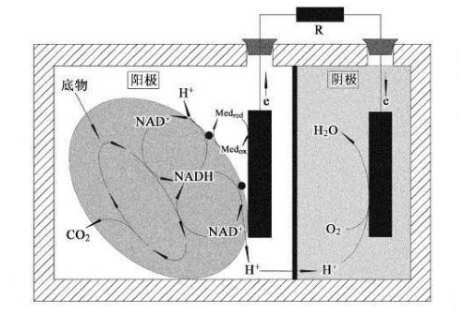
\includegraphics[width=0.6\textwidth]{figure/battery.png}
  \caption{微生物燃料电池示意图}
\end{figure}

\begin{figure}[H]
  \centering
  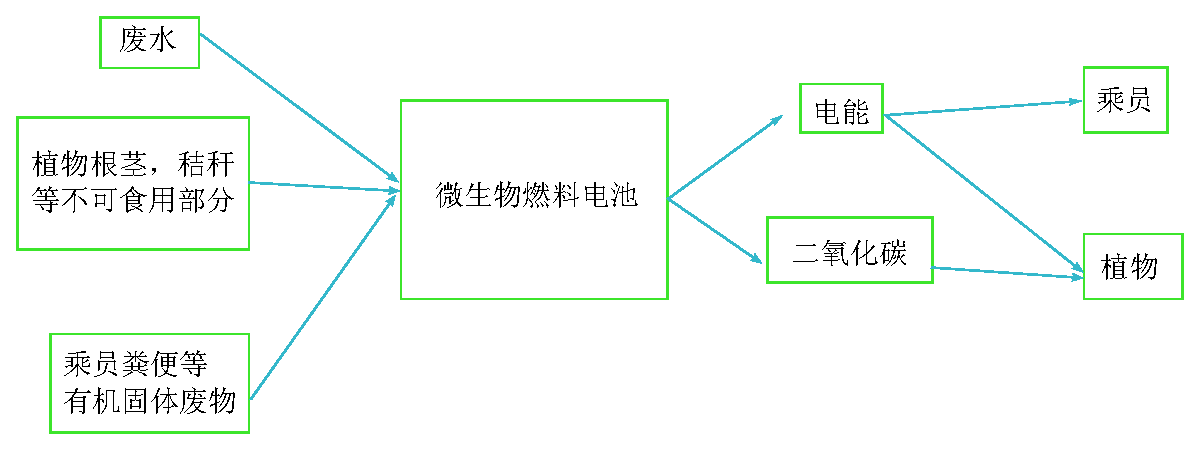
\includegraphics[width=\textwidth]{figure/recycling.eps}
  \caption{微生物燃料电池处理示意图}
\end{figure}

\section{电池材料的选择}

阳极:
从MFC的构成来看,阳极担负着微生物附着并传递电子的作用,它决定MFC产电能力的重要因素,同时也是研究微生物产电机理与电子传递机理的重要辅助工具,所以MFC阳极主要是以碳为主要材料,包括碳纸、碳布、石墨棒、碳毡、泡沫石墨以及碳纤维刷。

阳极是微生氧化分解有机物的场所,所以微生物的量也就能影响产电量。因此阳极材料的选择主要就是考虑材料的比表面积,此外,阳极除了材料还有就是阳极附着的微生物,如希瓦菌、假单胞菌、泥细菌等。但是在应用范围内,很少使用纯菌,而多数使用的为混合菌群。相较与纯菌,混合菌具有阻抗环境冲击能力强、利用基质范围广、降解底物速率和能量输出效率高的优点。

膜:
质子透过材料可以是盐桥,也要以是多孔的瓷隔膜,理想的材料是只允许质子透过,而基质、细菌和氧气等都被截留的微孔材料。我们选用的是质子交换膜PEM。

阴极:
阴极是制约MFC产电的主要原因之一。最理想的阴极电子受体应当是氧气,但是从氧气的还原动力学来看,氧气的还原速度较慢,这直接影响了MFC的产电性能。于是我们在阴极加入各种催化剂来提高氧气的还原速率。根据阴极催化剂的种类可以将MFC阴极分为非生物阴极和生物阴极。我们考虑选取生物阴极作为MFC的阴极。

非生物阴极:优点:氧气作为唯一电子受体,廉价易得。
缺点:石墨电极需要加入催化剂,铂电极昂贵、易使催化剂中毒失效。
生物阴极:优点:无需加入重金属催化材料和电子传递介质、不会引起催化剂中毒。
缺点:产生的电流不稳定(暂不用作主力供电)。

\section{备选方案}

固体废物采用高温好氧发酵处理,处理后的产物可以作为有机肥施用,发酵过程中产生的二氧化碳也可以通入植物舱,作为植物光合作用的原料。固体废物的处理及利用过程如下:首先,筛选高温好氧微生物菌群,该菌群可以降解植物秸秆中的纤维素,降解效率越高产生的二氧化碳越多,有机肥腐熟程度越高,也对植物种植越有利。所以微生物菌群的筛选对实验的顺利开展至关重要。另外,微生物接种比例要保持在合适的水平,一般接种菌剂比例在5\%到10\%之间。其次,按照堆肥适宜的碳氮比(一般30:1或35:1)计算乘员粪便和植物不可食部分合适的混合比例。其中,植物不可食部分主要为各种植物的秸秆和根类,进入发酵设备之前,首先将其移入综合舱内的储藏室晾干,再用植物粉碎机进行粉碎(为了保证发酵良好的通气性,一般粉碎粒径为2--20 \si{\milli\metre} )。最后,将固废混合物加入到固废转化器中,调节初始含水率50\%--70\%,温度50--60 \si{\degreeCelsius},并定时搅拌和通气。

\begin{figure}[H]
\label{chp:recycling:end}
  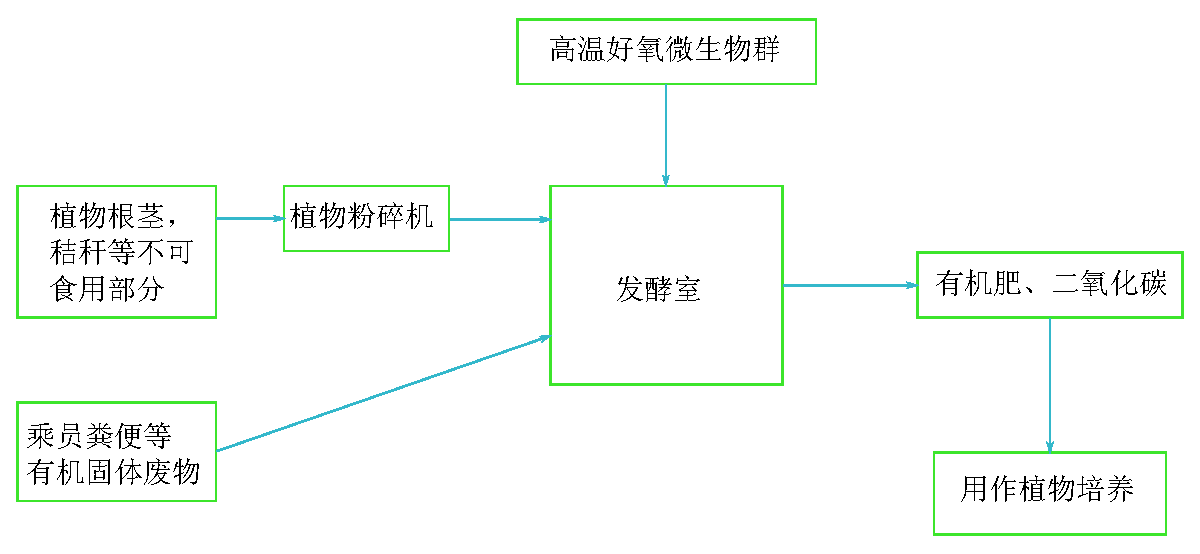
\includegraphics[width=0.8\textwidth]{figure/fajiao.eps}
  \centering
  \caption{发酵处理示意图}
\end{figure}
